%\documentclass{clases}
\documentclass[a4paper,12pt, oneside]{book}
\LoadClass[a4paper,12pt, oneside]{book}
\usepackage[skins,minted]{tcolorbox}
\usepackage[utf8]{inputenc}
\usepackage[T1]{fontenc}
\usepackage[spanish]{babel}
\languageshorthands{spanish}
\usepackage[numbers]{natbib}
%\usepackage{morewrites}
\usepackage{inconsolata}
\usepackage{mdframed}
\usepackage{minted}
\usepackage{listings}
\usepackage{subcaption}
\usepackage{amsmath}
\usepackage{amssymb}
\usepackage{graphicx, import}
\usepackage{hyperref}
\usepackage{longtable}
\usepackage{xcolor}
\usepackage{pdfpages}
%\usepackage{color}
\usepackage{fancyhdr}
\usepackage{menukeys}
\usepackage{appendix}
\usepackage{fontawesome}
\usepackage{comment}
\usepackage{caption}
\usepackage{setspace}
\usepackage[explicit]{titlesec}
\usepackage[a4paper]{geometry}
\geometry{top=3cm, bottom=3cm, left=4cm, right=2cm}
%\usepackage[draft]{listofsymbols}
%\usepackage[toc,acronym]{glossaries}
%\makeglossaries
%\glossarystyle{altlistgroup}

% se incluye el archivo de definición de acrónimos
%\include{acronimos}

% se incluye el archivo de definición de glsario
%\include{glosario}

%\opensymdef
%\input{capitulos/A2_simbolos}
%\closesymdef

\definecolor{green1}{HTML}{1dae28}
\definecolor{green2}{HTML}{afd095}
\definecolor{lightgray}{gray}{0.9}
\definecolor{orange}{RGB}{18,84,183}
\definecolor{titulo}{gray}{0.75}
\definecolor{gray97}{gray}{.97}
\definecolor{gray75}{gray}{.75}
\definecolor{gray45}{gray}{.45}
\definecolor{advertencia}{RGB}{255,178,102}
\definecolor{colorturqueza}{RGB}{178,223,238}
\definecolor{mintedbackground}{rgb}{0.95,0.95,0.95}
\definecolor{lbcolor}{rgb}{0.95,0.95,0.95}
\definecolor{mintedframe}{rgb}{0.0,0.0,0.0}
\lstset{
	frame=Ltb,
	tabsize=2,
	framerule=0pt,
	aboveskip=0.5cm,
	framextopmargin=0pt,
	framexbottommargin=0pt,
	framexleftmargin=0.4cm,
	framesep=0pt,
	rulesep=.0pt,
	backgroundcolor=\color{gray97},
	rulesepcolor=\color{blue},
	%
	stringstyle=\ttfamily,
	showstringspaces = false,
	basicstyle=\small\ttfamily,
	commentstyle=\color{gray45},
	keywordstyle=\bfseries,
	%
	numbers=none,
	numbersep=15pt,
	numberstyle=\tiny,
	numberfirstline = false,
	breaklines=true
}

\setminted[bash]{
	bgcolor=mintedbackground,
	fontfamily=tt,
	linenos=true,
	numberblanklines=true,
	numbersep=11pt,
	numbersep=2pt,
	gobble=0,
	frame=leftline,
	framesep=2mm,
	funcnamehighlighting=false,
	tabsize=4,
	obeytabs=false,
	samepage=false,
	showspaces=false,
	showtabs =false,
	texcl=false,
	baselinestretch=1.2,
	fontsize=\footnotesize,
	breaklines=true,
	breaksymbolleft=\ 
}


% minimizar fragmentado de listados
%\lstnewenvironment{listing}[1][]{\lstset{#1}\pagebreak[0]}{\pagebreak[0]}


\lstdefinestyle{consola}{
	basicstyle=\footnotesize\bf\ttfamily,
	backgroundcolor=\color{gray75},
}	
\definecolor{gray}{rgb}{0.4,0.4,0.4}
\definecolor{darkblue}{rgb}{0.0,0.0,0.6}
\definecolor{cyan}{rgb}{0.0,0.6,0.6}
\lstset{language=XML}

\lstdefinelanguage{XML}{
	morestring=[b]",
	tabsize=2,
	breaklines=true,
	morestring=[s]{>}{<},
	morecomment=[s]{<?}{?>},
	stringstyle=\color{black},
	identifierstyle=\color{darkblue},
	keywordstyle=\color{cyan},
	numbers=left,
	morekeywords={xmlns,version,type}% list your attributes here
}

\lstdefinestyle{C}{language=C}
\lstdefinestyle{XML}{language=XML}
\definecolor{codebg}{rgb}{0.96,0.96,0.96}
\definecolor{colorurls}{RGB}{107,17,17}
\definecolor{colorsql}{RGB}{255,245,245}
\definecolor{colorreferences}{RGB}{48,134,3}
\definecolor{titulo}{gray}{0.65}			%------ color para fondo del titulo de tablas.
\hypersetup{
	%bookmarks=true,         % show bookmarks bar?
	unicode=false,          % non-Latin characters in Acrobat’s bookmarks
	pdftoolbar=true,        % show Acrobat’s toolbar?
	pdfmenubar=true,        % show Acrobat’s menu?
	pdffitwindow=false,     % window fit to page when opened
	pdfstartview={FitH},    % fits the width of the page to the window
	pdftitle={Diseño de modelo para simulación 3D de VANT tipo cuadricóptero},    % title
	pdfauthor={Jesús Iván Medina Gil Lamadrid},     % author
	pdfsubject={Reporte final de residencias},   % subject of the document
	%pdfcreator={pdfTeX 3.14159265-2.6-1.40.16 (TeX Live 2016/dev)},   % creator of the document
	%pdfproducer={Panel HJ 2017}, % producer of the document
	pdfkeywords={simulación} {quadrotor} {vant} {ros} {gazebo} {hector\_quadrotor}, % list of keywords
	%pdfnewwindow=true,      % links in new PDF window
	colorlinks=true,       % false: boxed links; true: colored links
	linkcolor=black,          % color of internal links (change box color with linkbordercolor)
	citecolor=colorreferences,        % color of links to bibliography
	filecolor=magenta,      % color of file links
	urlcolor=blue,           % color of external links
	linkbordercolor={0 0 0}
}

\lstset{literate=
	{á}{{\'a}}1 {é}{{\'e}}1 {í}{{\'i}}1 {ó}{{\'o}}1 {ú}{{\'u}}1
	{Á}{{\'A}}1 {É}{{\'E}}1 {Í}{{\'I}}1 {Ó}{{\'O}}1 {Ú}{{\'U}}1
	{à}{{\`a}}1 {è}{{\`e}}1 {ì}{{\`i}}1 {ò}{{\`o}}1 {ù}{{\`u}}1
	{À}{{\`A}}1 {È}{{\'E}}1 {Ì}{{\`I}}1 {Ò}{{\`O}}1 {Ù}{{\`U}}1
	{ä}{{\"a}}1 {ë}{{\"e}}1 {ï}{{\"i}}1 {ö}{{\"o}}1 {ü}{{\"u}}1
	{Ä}{{\"A}}1 {Ë}{{\"E}}1 {Ï}{{\"I}}1 {Ö}{{\"O}}1 {Ü}{{\"U}}1
	{â}{{\^a}}1 {ê}{{\^e}}1 {î}{{\^i}}1 {ô}{{\^o}}1 {û}{{\^u}}1
	{Â}{{\^A}}1 {Ê}{{\^E}}1 {Î}{{\^I}}1 {Ô}{{\^O}}1 {Û}{{\^U}}1
	{œ}{{\oe}}1 {Œ}{{\OE}}1 {æ}{{\ae}}1 {Æ}{{\AE}}1 {ß}{{\ss}}1
	{ç}{{\c c}}1 {Ç}{{\c C}}1 {ø}{{\o}}1 {å}{{\r a}}1 {Å}{{\r A}}1
	{€}{{\EUR}}1 {£}{{\pounds}}1 {'}{{\textquotesingle}}1 {Ñ}{{\~N}}1
	{ñ}{{\~n}}1
}

\newtcblisting{terminal}[2][]{
	listing engine=minted,
	listing only,
	#1,
	title=#2,
	minted language=bash,
	colback=mintedbackground,
	top=0mm,
	bottom=0mm
}

\newtcblisting{consolestyle}[2][]{enhanced, listing engine=minted, 
	listing only,#1, title=#2, minted language=bash, 
	coltitle=mintedbackground!35!black, 
	fonttitle=\ttfamily\footnotesize,
	sharp corners, top=0mm, bottom=0mm,
	title code={\path[draw=mintedframe, dashed, fill=mintedbackground](title.south west)--(title.south east);},
	frame code={\path[draw=mintedframe, fill=mintedbackground](frame.south west) rectangle (frame.north east);}
}
\newenvironment{doble}
{\doublespacing
}

%\newcounter{comando}[section]
%\newenvironment{comando}[1][]{\refstepcounter{comando}\par\medskip
%	\noindent \textbf{Comando~\thecomando. #1} \rmfamily}{\medskip}
%\begin{terminal}{#1}
	
%\end{terminal}
%}{\medskip}

\graphicspath{ {img/} }

\begin{document}
	% Aquí se encuentra el archivo con la portada
	\begin{titlepage}
	\centering
	%-------------------------------------------
	% Logos en una tabla: izquierda, centro y derecha
	\begin{tabular}{@{}p{0.3\textwidth} p{0.3\textwidth} p{0.3\textwidth}@{}}
		
\includegraphics[height=2cm]{tecnm} & 
		\centering 
\includegraphics[height=1.5cm]{SEP} & 
		\raggedleft 
\includegraphics[height=2cm]{ith.jpg} \\
	\end{tabular}
	
	\vspace{2em}
	
	\noindent
	%-------------------------------------------
	%	Información institucional y académica (esquina superior izquierda)
	\begin{minipage}[t]{0.48\textwidth}
		\raggedright
		\small \textbf{%
			Instituto Tecnológico de Hermosillo\\
			Materia: Robótica\\
			Profesor: Medina Gil Lamadrid, Jesús Iván%
		}
	\end{minipage}%
	\hfill
	%	fecha actual (esquina superior derecha), en letras pequeñas y en negrita.
	\begin{minipage}[t]{0.48\textwidth}
		\raggedleft
		\small \textbf{\today}
	\end{minipage}
	
	\vspace{2em}
	
	%-----------------------------------------
	% Unidad y Título de la tarea en letras grandes y en negrita
	{\large \textbf{Unidad 1: Morfología del robot}}\\
	{\Huge \textbf{Tipos de Sensores}}
		
	\vspace{1em}
	
	%---------------------------------------
	% Tabla con la información del equipo
	%---------------------------------------
	% Encabezado del equipo
	\begin{center}
		{\Large \textbf{Equipo 2}}
	\end{center}
	
	\vspace{1em}
	
	% Tabla de integrantes:
	% Cada fila contiene: foto (columna izquierda) y datos del integrante (columna derecha)
	\begin{center}
		\begin{tabular}{c c}
			\begin{tabular}{c}
				
\includegraphics[height=3cm]{Cedano.jpeg} \\
				\textbf{Cedano Mendoza},\\ Carlos Francisco \\ \texttt{L21330552@hermosillo.tecnm.mx} \\ Teléfono: 6624686707
			\end{tabular} &
			\begin{tabular}{c}
				
\includegraphics[height=3cm]{Martinez.png} \\
				\textbf{Martinez Navarro,}\\ Sebastian \\ \texttt{L2133} \\ Teléfono: 6621053764
			\end{tabular} \\ \vspace{2em}
			\begin{tabular}{c}
				
\includegraphics[height=3cm]{Ocampo.jpeg} \\
				\textbf{Ocampo Ramos,}\\ Addiel Adrián \\ \texttt{L20330895@hermosillo.tecnm.mx} \\ Teléfono: 6623501716
			\end{tabular} &
			\begin{tabular}{c}
				\includegraphics[height=3cm]{Pérez.jpeg} \\
				\textbf{Pérez Estupiñán,}\\ Ana Claudia \\ \texttt{L21330669@hermosillo.tecnm.mx} \\ Teléfono: 6624281154
			\end{tabular}
		\end{tabular}
	\end{center}

\end{titlepage}

	\onehalfspacing
	\frontmatter
	\pagestyle{plain}  % numeración en páginas preliminares
	\titleformat{\chapter}
	{\bfseries\huge}
	{}
	{0pt}
	{~\raisebox{-1.5pt}{}
	\\\filleft #1 \\\vspace{.25cm}\titlerule[1.5pt]}
	
	% ---------------------------------------
	% índices
%	\clearpage   % o \cleardoublepage, según prefieras
	\newpage
	\phantomsection    % crea un nuevo destino para hyperref
	\addcontentsline{toc}{chapter}{Índice general}
	\tableofcontents
	
%	\clearpage
	\newpage
	\phantomsection
	\addcontentsline{toc}{chapter}{Índice de figuras}
	\listoffigures
	
	\hypersetup{
		linkcolor=red
	}
	
	% ---------------------------------------
	% Estilo de encabezado y pie de página
	\mainmatter
	\pagestyle{fancy}
	\fancyhead{}
	\fancyhead[L]{\leftmark}
	\fancyhead[R]{}
	\fancyfoot[L]{\parbox[l]{\textwidth-1cm}{\rightmark}}
	\fancyfoot[C]{}
	\fancyfoot[R]{\thepage}
	\renewcommand{\footrulewidth}{0.5pt}
	%\fancyfoot[RO,LE]{Diseño de modelo para simulación 3D de VANT tipo cuadricóptero}
	
	\titleformat{\chapter}
	{\bfseries\huge}
	{}
	{0pt}
	{\titlerule[3pt]~\raisebox{-1.5pt}{\sc{\chaptername}~\thechapter}~\titlerule[3pt]%
		\\\vspace{.05cm}\titlerule\\\filcenter #1 \\\vspace{.25cm}\titlerule}
	
	% Capítulo 1: Introducción
	\chapter{Introducción} \label{chap:introduccion}

En este capítulo, se explica un pequeño resumen del reporte. Los temas que se verán y explicar un poco sobre su robot sin entrar en muchos detalles.

Cabe destacar que si no quieren escribir algún capítulo, con \TeX studio pueden comentar la línea (O las líneas seleccionadas) con \menu{Ctrl} + \menu{T}, mientras que para descomentar la línea es el mismo comando.

También si presionan \menu{Ctrl} y luego hacen \menu{Clic Izquierdo} en el documento que se muestra a la derecha (después de presionar \menu{compilar y ver} o \menu{F5}), podrán abrir esa parte del código de \LaTeX. Pueden hacer lo mismo en el código para entrar a esa parte del documento o usar \menu{Ctrl} + \menu{Clic Izquierdo}.

También si quieren modificar la bibliografía, solo tienen que abrir el archivo llamado bibliografia.bib o ir al final del archivo principal, \ffile{Reporte.tex}, donde dice

\begin{latexcode}{\LaTeX}
		% Pulsa Ctrl + Clic Izquierdo en bibliografia para entrar.
		\bibliography{bibliografia}
	\end{document}
\end{latexcode}

Por último, recuerden que este formato está basado en la perfección. Y uno no puede entregar la perfección cuando queda menos de una semana para entregar la tarea y hay temas que ni completamos, así que no es necesario completarlo todo.
	
	% Capítulo 2: Marco Teórico
	\chapter{Introducción} \label{chap:introduccion}

En este capítulo, se explica un pequeño resumen del reporte. Los temas que se verán y explicar un poco sobre su robot sin entrar en muchos detalles.

Cabe destacar que si no quieren escribir algún capítulo, con \TeX studio pueden comentar la línea (O las líneas seleccionadas) con \menu{Ctrl} + \menu{T}, mientras que para descomentar la línea es el mismo comando.

También si presionan \menu{Ctrl} y luego hacen \menu{Clic Izquierdo} en el documento que se muestra a la derecha (después de presionar \menu{compilar y ver} o \menu{F5}), podrán abrir esa parte del código de \LaTeX. Pueden hacer lo mismo en el código para entrar a esa parte del documento o usar \menu{Ctrl} + \menu{Clic Izquierdo}.

También si quieren modificar la bibliografía, solo tienen que abrir el archivo llamado bibliografia.bib o ir al final del archivo principal, \ffile{Reporte.tex}, donde dice

\begin{latexcode}{\LaTeX}
		% Pulsa Ctrl + Clic Izquierdo en bibliografia para entrar.
		\bibliography{bibliografia}
	\end{document}
\end{latexcode}

Por último, recuerden que este formato está basado en la perfección. Y uno no puede entregar la perfección cuando queda menos de una semana para entregar la tarea y hay temas que ni completamos, así que no es necesario completarlo todo.
	
		\section{Cinemática} \label{sec:cinematica}

Explicar su definición en base a lo que viene en libros o de los archivos de Matlab. Diferenciar entre \textbf{Cinemática directa} y \textbf{Cinemática inversa}.
Para el proceso sobre cómo se llevó a cabo el algoritmo en Matlab, ir a la  \hyperref[sec:proceso_cinematica]{sección del proceso de Cinemática}.

\subsection{Cinemática Directa}
Explicar sobre la definición geométrica usando Denavit Hartenberg con el algoritmo y las matemáticas.

\subsection{Cinemática Diferencial}
Aquí explicarán sobre el jacobiano para la cinemática diferencial.

\subsection{Cinemática Inversa}
Explicar su definición y cómo se relaciona el gradiente con el jacobiano. Cabe destacar que existen multitud de métodos y en mi clase solo usaron un método, pero aquí pueden explicar las imágenes que vienen en Matlab.


		
		\section{ROS} \label{sec:ros}
Aquí se explicará un poco sobre qué es ROS.
\begin{figure}[h]
	\centering
	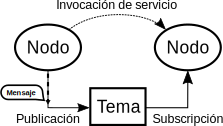
\includegraphics[width=0.5\linewidth]{img/ROS_concepts}
	\caption{Diagrama de comunicación de ROS}
	\label{fig:rosconcepts}
\end{figure}

También están interesantes las animaciones que vienen en la \href{https://docs.ros.org/en/humble/Tutorials/Beginner-CLI-Tools/Understanding-ROS2-Topics/Understanding-ROS2-Topics.html}{página de ROS} \cite{ros2-understanding-topics}, pero lamentablemente no se pueden poner animaciones en el reporte.

\subsection{Nodo (Node)}
\subsection{Tema (Topic)}
\subsection{Mensaje (Message)}
\subsection{Servicio (Service)}
\subsection{Gazebo}
\subsection{RViz}

		
		\section{Dinámica} \label{sec:dinamica}

Se refiere al estudio de cómo las fuerzas afectan el movimiento de un robot. Mientras que la cinemática se enfoca en el movimiento sin considerar sus causas, la dinámica incorpora elementos como la masa, la aceleración, la fricción y fuerzas externas. Para un manipulador, se considera tanto la velocidad lineal y angular de cada eslabón como las fuerzas y torques que intervienen\cite{Barrientos_fundamentos_robotica}.

La velocidad del centro de masa de un eslabón \(i\) está compuesta por una parte lineal y otra angular, dependiendo del tipo de articulación del robot. Para una articulación revoluta, la velocidad angular es \(\dot{q}_i\), mientras que para una prismática, lo es la velocidad lineal \(\dot{q}_i\). Estas velocidades pueden expresarse en función de las velocidades articulares mediante el Jacobiano:

\begin{equation}
	\mathbf{v}_i = \mathbf{J}_{v_i}(\mathbf{q}) \dot{\mathbf{q}}, \quad
	\boldsymbol{\omega}_i = \mathbf{J}_{\omega_i}(\mathbf{q}) \dot{\mathbf{q}} \text{\cite{Barrientos_fundamentos_robotica}}.
\end{equation}


donde \(\mathbf{J}_{v_i}\) y \(\mathbf{J}_{\omega_i}\) son las matrices jacobianas lineal y angular, respectivamente.

El tensor de inercia \(\mathbf{I}_i\) describe cómo está distribuida la masa del eslabón \(i\) respecto a su centro de masa, y afecta directamente la dinámica rotacional del sistema.

En general, el modelo dinámico de un robot puede representarse como:

\begin{equation}
	\boldsymbol{\tau} = \boldsymbol{\tau}_{motor} - \boldsymbol{\tau}_{perturb} - \boldsymbol{\tau}_{fric\_din} - \boldsymbol{\tau}_{fric\_est}
\end{equation}

donde:
\begin{itemize}
	\item \(\boldsymbol{\tau}_{motor}\) son los torques generados por los motores,
	\item \(\boldsymbol{\tau}_{perturb}\) representan perturbaciones externas,
	\item \(\boldsymbol{\tau}_{fric\_din}\) corresponde a la fricción dinámica o viscosa,
	\item \(\boldsymbol{\tau}_{fric\_est}\) es la fricción estática o seca.
\end{itemize}

El modelo dinámico estándar con \(n\) grados de libertad se puede expresar mediante la siguiente ecuación:

\begin{equation}
	\mathbf{M}(\mathbf{q}) \ddot{\mathbf{q}} + \mathbf{C}(\mathbf{q}, \dot{\mathbf{q}}) \dot{\mathbf{q}} + \mathbf{g}(\mathbf{q}) = \boldsymbol{\tau}
\end{equation}

donde:
- \(\mathbf{M}(\mathbf{q})\) es la matriz de masa o inercia,
- \(\mathbf{C}(\mathbf{q}, \dot{\mathbf{q}})\) representa los efectos de Coriolis y centrífugos,
- \(\mathbf{g}(\mathbf{q})\) es el vector de fuerzas gravitacionales,
- \(\boldsymbol{\tau}\) es el vector de torques o fuerzas aplicadas en las articulaciones.

Para obtener este modelo, se pueden utilizar distintos métodos, entre los que destacan:

\begin{itemize}
	\item \textbf{Método de Euler-Lagrange:} basado en la formulación energética del sistema, utilizando energía cinética y potencial para derivar las ecuaciones de movimiento.
	\item \textbf{Método de Newton-Euler:} aplica las leyes del movimiento de Newton de forma recursiva en cada eslabón, considerando las fuerzas y torques internos y externos.
\end{itemize}


\subsection{Matriz de masa o inercia}

Esta matriz representa cómo la masa del robot está distribuida en sus diferentes partes y cómo esa distribución afecta el movimiento.Esta depende de la configuración del robot y de sus parámetros físicos (longitudes, masas, centros de masa, etc.). En términos simples, determina cuánta fuerza se necesita para generar una aceleración en cada articulación. Cuanto mayor sea el valor de esta matriz, más difícil será acelerar el movimiento del robot.\cite{Barrientos_fundamentos_robotica}.

En un robot con \(n\) articulaciones, la matriz de masa \(\mathbf{M}(\mathbf{q})\) es definida positiva y de tamaño \(n \times n\). Se construye sumando las contribuciones cinéticas de cada eslabón, considerando su masa \(m_i\), su centro de masa y su inercia rotacional:

\begin{equation}
	\mathbf{M}(\mathbf{q}) = \sum_{i=1}^n \left( m_i \mathbf{J}_{v_i}^T \mathbf{J}_{v_i} + \mathbf{J}_{\omega_i}^T \mathbf{R}_i \mathbf{I}_i \mathbf{R}_i^T \mathbf{J}_{\omega_i} \right)
	\text{\cite{Pearson_robot}}
\end{equation}

donde:
\begin{itemize}
	\item \(\mathbf{J}_{v_i}, \mathbf{J}_{\omega_i}\): Jacobianos lineal y angular del eslabón \(i\),
	\item \(\mathbf{R}_i\): matriz de rotación del sistema del eslabón al sistema inercial,
	\item \(\mathbf{I}_i\): tensor de inercia del eslabón \(i\) respecto a su centro de masa,
	\item \(m_i\): masa del eslabón \(i\).
\end{itemize}

---

\subsection{Matriz de Coriolis}

La matriz de Coriolis incluye términos que dependen de la velocidad de las articulaciones y representan fuerzas que aparecen debido al movimiento conjunto de las distintas partes del robot. Estas fuerzas pueden actuar como una especie de resistencia o interferencia entre articulaciones en movimiento. Aunque su cálculo es complejo, su efecto puede visualizarse como una “fuerza ficticia” que aparece cuando el robot está girando o moviéndose rápidamente.

Una forma común de calcular la matriz de Coriolis \(\mathbf{C}(\mathbf{q}, \dot{\mathbf{q}})\) es mediante los **coeficientes de Christoffel**:

\begin{equation}
	c_{ijk} = \frac{1}{2} \left( \frac{\partial m_{ij}}{\partial q_k} + \frac{\partial m_{ik}}{\partial q_j} - \frac{\partial m_{jk}}{\partial q_i} \right)
\end{equation}

Entonces, los elementos de la matriz se construyen así:

\begin{equation}
	C_{ij} = \sum_{k=1}^n c_{ijk} \dot{q}_k
\end{equation}

Y el torque total por efectos de Coriolis es:

\begin{equation}
	\boldsymbol{\tau}_{coriolis} = \mathbf{C}(\mathbf{q}, \dot{\mathbf{q}})\dot{\mathbf{q}}
\end{equation}



\subsection{Vector de gravedad}

El vector de gravedad representa las fuerzas gravitatorias que actúan sobre las articulaciones del robot dependiendo de su configuración. Estas fuerzas cambian según la orientación del robot en el espacio. Por ejemplo, cuando el robot está completamente extendido de forma horizontal, el peso de sus partes genera un mayor torque sobre las articulaciones. Es por eso que en esa posición, los motores deben aplicar mayor fuerza para sostener al robot y evitar que caiga por efecto de la gravedad.

Se expresa como:

\begin{equation}
	\mathbf{g}(\mathbf{q}) = \sum_{i=1}^n m_i \mathbf{J}_{v_i}^T \mathbf{g}_0
\end{equation}

donde:
\begin{itemize}
	\item \(\mathbf{g}_0\) es el vector de gravedad en el marco base, típicamente \([0, 0, -g]^T\),
	\item \(\mathbf{J}_{v_i}\) es el Jacobiano lineal del centro de masa del eslabón \(i\),
	\item \(m_i\) es la masa del eslabón \(i\).
\end{itemize}




\subsection{Fricción}

La fricción es una fuerza que se opone al movimiento y puede ser modelada en robótica como una suma de componentes estática (seca) y dinámica (viscosa).

\subsubsection{Fricción estática o seca}

Se modela como un torque constante que debe superarse para iniciar el movimiento. Su modelo ideal es discontinuo:

\begin{equation}
	\boldsymbol{\tau}_{fric\_est} = \mathbf{K}_s \cdot \text{sign}(\dot{\mathbf{q}})
\end{equation}

donde \(\mathbf{K}_s\) contiene los coeficientes de fricción estática por articulación.

\subsubsection{Fricción dinámica o viscosa}

 Aparece cuando las partes del robot ya están en movimiento. Es proporcional a la velocidad y actúa como una resistencia que disipa energía. Este tipo de fricción es útil para estabilizar movimientos, ya que suaviza el comportamiento del robot al frenar movimientos demasiado rápidos o bruscos.

Se modela como proporcional a la velocidad articular:

\begin{equation}
	\boldsymbol{\tau}_{fric\_din} = \mathbf{K}_v \dot{\mathbf{q}}
\end{equation}

donde \(\mathbf{K}_v\) es una matriz diagonal con los coeficientes de fricción viscosa.



\subsection{Perturbaciones}

Las perturbaciones son fuerzas o efectos externos que no se pueden controlar ni predecir completamente, como golpes, viento, errores en los sensores, o variaciones en el peso del objeto que el robot manipula. Aunque no siempre se modelan en detalle, es importante tenerlas en cuenta al diseñar controladores robustos que permitan al robot seguir funcionando correctamente frente a estas situaciones inesperadas.


Se modelan generalmente como un término adicional en la ecuación dinámica:

\begin{equation}
	\boldsymbol{\tau}_{perturb} = \boldsymbol{\tau}_{ext} + \Delta\boldsymbol{\tau}
\end{equation}

donde \(\Delta\boldsymbol{\tau}\) representa errores de modelado o influencias no previstas. 

		
		\section{Control}
Si quieren, pueden comentar esta parte, pero si quieren, expliquen el diagrama de bloques de la \autoref{fig:diagrama-de-robot-industrial}.

\begin{figure}[h]
	\centering
	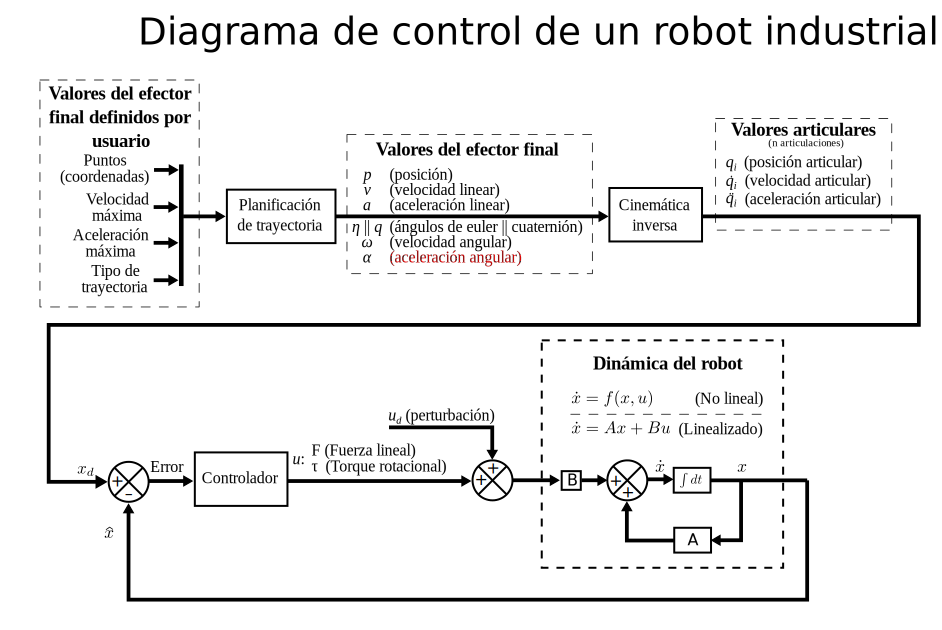
\includegraphics[width=\linewidth]{img/Diagrama_robot_industrial}
	\caption{Diagrama de bloques de un robot industrial}
	\label{fig:diagrama-de-robot-industrial}
\end{figure}

	
	% Capítulo 3: Desarrollo
	\chapter{Introducción} \label{chap:introduccion}

En este capítulo, se explica un pequeño resumen del reporte. Los temas que se verán y explicar un poco sobre su robot sin entrar en muchos detalles.

Cabe destacar que si no quieren escribir algún capítulo, con \TeX studio pueden comentar la línea (O las líneas seleccionadas) con \menu{Ctrl} + \menu{T}, mientras que para descomentar la línea es el mismo comando.

También si presionan \menu{Ctrl} y luego hacen \menu{Clic Izquierdo} en el documento que se muestra a la derecha (después de presionar \menu{compilar y ver} o \menu{F5}), podrán abrir esa parte del código de \LaTeX. Pueden hacer lo mismo en el código para entrar a esa parte del documento o usar \menu{Ctrl} + \menu{Clic Izquierdo}.

También si quieren modificar la bibliografía, solo tienen que abrir el archivo llamado bibliografia.bib o ir al final del archivo principal, \ffile{Reporte.tex}, donde dice

\begin{latexcode}{\LaTeX}
		% Pulsa Ctrl + Clic Izquierdo en bibliografia para entrar.
		\bibliography{bibliografia}
	\end{document}
\end{latexcode}

Por último, recuerden que este formato está basado en la perfección. Y uno no puede entregar la perfección cuando queda menos de una semana para entregar la tarea y hay temas que ni completamos, así que no es necesario completarlo todo.
	
		\section{Características del Robot} \label{sec:caracteristicas_del_robot}

El robot utilizado en este proyecto es un manipulador articulado de varios grados de libertad, cuya estructura fue previamente dise\~nada en SolidWorks. Este tipo de robot est\'a compuesto por una serie de eslabones y articulaciones conectadas en serie, lo que le permite alcanzar una variedad de posiciones y orientaciones en el espacio tridimensional.

\begin{figure}[H]
	\centering
	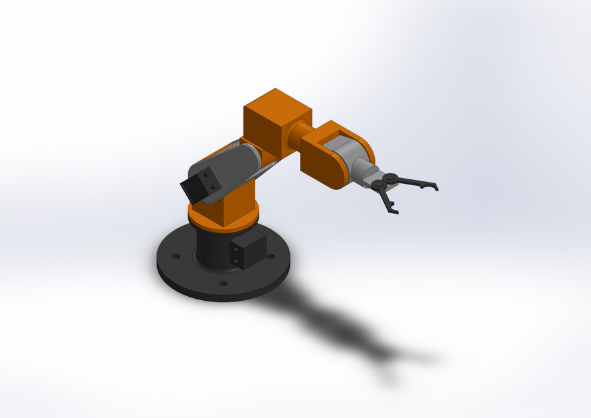
\includegraphics[width=0.7\textwidth]{caracteristicas del robot}
	\caption{Características del robot utilizado en el proyecto.}
	\label{fig:caracteristicas_robot}
\end{figure}


	La tabla de Denavit-Hartenberg (DH) es una herramienta fundamental para describir la geometría cinemática de un robot manipulador. Esta tabla resume los parámetros geométricos necesarios para modelar la posición y orientación relativa entre los eslabones adyacentes del robot.
\begin{table}[ht]

	\centering
	\caption{Parámetros de Denavit Hartenberg y límites del robot}
	\label{tab:parametros_robot}
	\begin{tabular}{ l|cccccccccccc
		}
		\toprule
		N & {$\theta$} & {$d$} & {$a$} & {$\alpha$} & {tipo} 
		& {$q_{\min}$} & {$q_{\max}$} 
		& {$\dot q_{\max}$} & {$\ddot q_{\max}$} 
		& {$\tau$} & {$\mu_s$} & {$\mu_k$} \\
		\midrule
		1 & 0 & 95 & 0  & -90   & r & -90 & 90 & 180 & 360 &  1.041  & 0.1 & 0.2 \\
		2 & -90 & 0 & 152  & 0 & r & -90 & 180 & 180 & 360 & 2.31  & 0.1 & 0.2 \\
		3 & 90 & 0 & 167  & 0 & r & -90 & 180 & 180 & 360 & 2  & 0.1 & 0.2 \\
		4 & -90 & 80 & 0  & -90   & r &   -90 &  180 &   180 &   360 & 0.6  & 0.1 & 0.2 \\
		\bottomrule
	\end{tabular}
\end{table}
\bigskip
\noindent
\begin{description}
	\item[N] Número de la articulación.
	\item[\(\theta\)] Ángulo articular (grados).
	\item[\(d\)] Desplazamiento articular (mm).
	\item[\(a\)] Longitud del eslabón (mm).
	\item[\(\alpha\)] Ángulo de torsión DH (grados).
	\item[tipo] ‘r’ para articulación rotacional, ‘p’ para prismática.
	\item[\(q_{\min}\), \(q_{\max}\)] Límites de posición (grados o mm).
	\item[\(\dot q_{\max}\)] Límite de velocidad (grados/s o m/s).
	\item[\(\ddot q_{\max}\)] Límite de aceleración (grados/s² o m/s²).
	\item[\(\tau\)] Torque o fuerza máxima permitido (\(N \cdot m\) o \(N\)).
	\item[\(\mu_s\)] Fricción estática (\(N\) o \(N \cdot m\)).
	\item[\(\mu_k\)] Fricción cinética (\(N \cdot m \cdot s\) o \(\frac{N \cdot m \cdot s}{rad}\)).
\end{description}


		
			\subsection{Partes} \label{subsec:partes} 

Para la construcción del brazo robótico se utilizaron motores y eslabones adecuados para soportar el peso del sistema y generar el movimiento requerido.

\textbf{Motores:} Se utilizaron dos tipos de actuadores principales:

\begin{itemize}
	\item \textbf{Motor DC MAXON RE40 con reductor planetario 100:1.} Este motor es compacto y robusto, ideal para aplicaciones de robótica que requieren alto torque y control preciso. Según su hoja de datos, puede entregar un torque continuo de hasta 63.6 mNm (antes del reductor), y su reductor planetario amplifica este torque en una proporción 100:1. Su velocidad máxima sin carga ronda los 8,000 rpm (que se reducen a 80 rpm tras el reductor), con una masa aproximada de 470 g. Este tipo de motor se empleó en articulaciones donde se requiere mayor velocidad y moderado torque.
	
	\item \textbf{Harmonic Drive FHA-C Mini Series, modelo FHA-25C-50-E250.} Este tipo de actuador integra motor, reductor armónico y encoder en un solo conjunto compacto. Ofrece una excelente precisión y bajo juego mecánico. El modelo FHA-25C-50-E250 tiene una relación de reducción de 50:1, un torque nominal de hasta 21 Nm y una resolución de encoder de hasta 250,000 pulsos por revolución. Se utilizó en articulaciones que requieren mayor precisión y torque constante.
\end{itemize}

Los torques máximos aplicados por cada articulación del brazo robótico son los siguientes:

\begin{itemize}
	\item \textbf{Articulación 1 (T1):} 0.694 Nm
	\item \textbf{Articulación 2 (T2):} 1.54 Nm
	\item \textbf{Articulación 3 (T3):} 1.33 Nm
	\item \textbf{Articulación 4 (T4):} 0.405 Nm
\end{itemize}

\textbf{Eslabones:} Todos los eslabones están fabricados en aluminio debido a su ligereza, resistencia y facilidad de mecanizado. A continuación, se describen las características de cada uno:

\begin{itemize}
	\item \textbf{Eslabón 1:} Masa de 770 g y longitud de 50 mm.
	\item \textbf{Eslabón 2:} Masa de 429 g y longitud de 152.75 mm.
	\item \textbf{Eslabón 3:} Masa de 762 g y longitud de 167 mm.
	\item \textbf{Eslabón 4:} Masa de 187 g y longitud de 95 mm.
\end{itemize}



			
			\subsection{Límites y propiedades dinámicas de las articulaciones} \label{subsec:limites_propiedades}

Básicamente, explicarán lo que aparece en la \autoref{tab:parametros_robot}: Parámetros de Denavit Hartenberg y límites del robot, específicamente lo que aparece después de \code{tipo}. Como no completamos la tarea de dinámica,. pueden comentar esta subsección del documento principal.
		
		\section{Proceso de Cinemática} \label{sec:proceso_cinematica}

Para el análisis del comportamiento del manipulador, se implementaron los procesos de cinemática utilizando herramientas de simulación en MATLAB, con base en la tabla de parámetros Denavit-Hartenberg (DH) desarrollada a partir del modelo CAD del robot.
Las simulaciones se llevaron a cabo empleando plantillas proporcionadas por el docente, adaptadas a la configuración específica del robot utilizado por el equipo.

A lo largo de esta sección, se llevaron a cabo simulaciones que permitieron obtener, visualizar y validar el comportamiento del efector final y de las articulaciones del robot frente a distintas trayectorias y configuraciones deseadas. Estos procesos resultaron fundamentales para garantizar que el modelo matemático del robot se comportara de forma coherente con su diseño físico.

El análisis se divide en tres etapas principales: cinemática directa, cinemática diferencial y cinemática inversa. Cada una de ellas se desarrolla en detalle en las secciones subsecuentes, junto con los resultados obtenidos y sus respectivas gráficas y animaciones.

\subsection{Cinemática Directa} \label{subsec:cinematica_directa}

La cinemática directa consiste en determinar la posición y orientación del efector final a partir de los valores de las variables articulares del robot. Para el brazo robótico en estudio, esta operación se basa en la tabla de parámetros Denavit-Hartenberg (DH) obtenida del modelo CAD, la cual permite construir las matrices de transformación homogénea necesarias para describir la configuración espacial del efector final.

Durante el desarrollo del proyecto, se utilizó como base un conjunto de scripts en \texttt{MATLAB} proporcionado por el profesor Jesús Iván Medina Gil Lamadrid, el cual se encuentra disponible públicamente en el repositorio de GitHub \cite{medinagl_robotica}. Este código facilitó la implementación de los modelos de cinemática directa, diferencial e inversa del manipulador.
 \\

Primero, se actualiza la configuración del robot con los valores articulares actuales:

\begin{matlabcode}{matlab}
	robot = actualizar_robot(robot, q(:,k));
\end{matlabcode}

Luego, se extraen la posición y la matriz de rotación del efector final:

\begin{matlabcode}{matlab}
	posicion(:,k) = robot.T(1:3,4,end);
	R(:,:,k) = robot.T(1:3,1:3,end);
\end{matlabcode}

A continuación, se obtiene la orientación en ángulos de Euler a partir de la matriz de rotación:

\begin{matlabcode}{matlab}
	orientacion(:,k) = rotMat2euler(R(:,:,k), secuencia);
\end{matlabcode}

Con la configuración actualizada, se calcula el Jacobiano geométrico:

\begin{matlabcode}{matlab}
	[Jv(:,:,k), Jw(:,:,k)] = jac_geometrico(robot);
\end{matlabcode}

Finalmente, se calculan la velocidad lineal y angular del efector final:

\begin{matlabcode}{matlab}
	vel_linear(:,k)  = Jv(:,:,k) * (q(:,k)/dt);
	vel_angular(:,k) = Jw(:,:,k) * (q(:,k)/dt);
\end{matlabcode}

Este procedimiento se repite para cada instante de tiempo para obtener la trayectoria completa del efector final.

Los resultados obtenidos con este procedimiento se presentan en la sección de Resultados, especificamente en la Figura~\ref{fig:CinematicaDirecta}.

%Para ver los resultados, ir al \autoref{chap:resultados}: Resultados, o determinada figura.
\subsection{Cinemática Diferencial}

La cinemática diferencial describe cómo se relacionan las velocidades articulares del robot con las velocidades lineales y angulares del efector final. Para ello, se utiliza el Jacobiano geométrico, que se compone de dos partes:
\begin{itemize}
	\item $J_v$: Parte traslacional.
	\item $J_w$: Parte rotacional.
\end{itemize}

A continuación se presenta el código que calcula el Jacobiano paso a paso, con su respectiva explicación.

Antes de comenzar, se extraen de la estructura del robot las matrices necesarias para calcular el Jacobiano: la transformación base, las transformaciones globales de cada articulación, el número de grados de libertad, y los tipos de articulaciones.

\begin{matlabcode}{matlab}
	function [Jv, Jw] = jac_geometrico(r)
	A0 = r.A0;
	T = r.T;
	NGDL = r.NGDL;
	tipo = r.tipo;
\end{matlabcode}

Se inicializan las matrices vacías para el Jacobiano traslacional ($J_v$) y rotacional ($J_w$), con ceros.

\begin{matlabcode}{matlab}
	Jv = zeros(3, NGDL);
	Jw = zeros(3, NGDL);
\end{matlabcode}

Se obtiene la posición final del efector desde la última transformación. También se definen el origen y el eje $z$ del sistema base, tomados desde la matriz $A0$.

\begin{matlabcode}{matlab}
	p_end = T(1:3, 4, end);
	p0 = A0(1:3, 4);
	z0 = A0(1:3, 3);
\end{matlabcode}

Se recorre cada articulación del robot. Si es la primera, se usa el sistema base como referencia; en caso contrario, se usa el marco anterior para calcular los vectores necesarios.

\begin{matlabcode}{matlab}
	for i = 1:NGDL
	if i == 1
	p_prev = p0;
	z_prev = z0;
	else
	p_prev = T(1:3, 4, i-1);
	z_prev = T(1:3, 3, i-1);
	end
\end{matlabcode}

Dependiendo del tipo de articulación (revoluta 'r' o prismática 'p'), se calcula la columna $i$ del Jacobiano de forma distinta:
\begin{itemize}
	\item Si es revoluta:
	\begin{itemize}
		\item $Jv(:,i) = z_{i-1} \times (p_{end} - p_{i-1})$.
		\item $Jw(:,i) = z_{i-1}$.
	\end{itemize}
	\item Si es prismática:
	\begin{itemize}
		\item $Jv(:,i) = z_{i-1}$.
		\item $Jw(:,i) = [0; 0; 0]$.
	\end{itemize}
\end{itemize}

\begin{matlabcode}{matlab}
	switch tipo(i)
	case 'r'
	Jv(:, i) = cross(z_prev, (p_end - p_prev));
	Jw(:, i) = z_prev;
	case 'p'
	Jv(:, i) = z_prev;
	Jw(:, i) = [0; 0; 0];
	otherwise
	error('Tipo de junta inválido, debe ser ''r'' o ''p''.');
	end
\end{matlabcode}

\subsection{Cinemática Inversa}

Para determinar las configuraciones articulares que permiten alcanzar posiciones deseadas del efector final, se implementa un método iterativo de cinemática inversa. A continuación se describen las partes principales del código:

\bigskip

Definición de parámetros para el método iterativo:

\begin{matlabcode}{matlab}
	tol = 1e-6;         % Tolerancia para el error en la posición
	max_iter = 100;     % Número máximo de iteraciones permitidas
	alpha = 1.0;        % Factor de corrección en cada iteración
	numSamples = 100;   % Número de configuraciones iniciales aleatorias
\end{matlabcode}

Estos parámetros controlan la precisión, límite de iteraciones y la cantidad de puntos de partida para la búsqueda de soluciones.

\bigskip

Inicialización de matrices para guardar las soluciones obtenidas:

\begin{matlabcode}{matlab}
	q_sol = zeros(robot.NGDL, n);   % Matriz para almacenar las soluciones articulares
	p_sol = zeros(3, n);            % Matriz para almacenar las posiciones calculadas
\end{matlabcode}

Aquí, \texttt{n} corresponde al número de puntos en la trayectoria deseada.

\bigskip

Cálculo iterativo de la cinemática inversa para cada punto de la trayectoria:

\begin{matlabcode}{matlab}
	for i = 1:n
	[q_sol(:,i), p_sol(:,i)] = cinematica_inv(robot, pos_puntos(:,i), tol, max_iter, alpha, numSamples);
	end
\end{matlabcode}

Se recorre cada posición deseada y se calcula la configuración articular correspondiente usando la función \texttt{cinematica\_inv}.

\bigskip

Generación de la trayectoria articular con perfil trapezoidal de velocidad:

\begin{matlabcode}{matlab}
	delta_q = abs(q_sol(:,2) - q_sol(:,1));
	t_final = max(2 * delta_q ./ robot.dqMax);
	numSamples = 201;
	[q, dq, ddq, t, pp] = trapveltraj(q_sol, numSamples, 'Acceleration', robot.ddqMax, 'EndTime', t_final);
\end{matlabcode}

Este bloque calcula un perfil suave para el movimiento articular entre las posiciones calculadas, respetando las velocidades y aceleraciones máximas.

\bigskip

Los resultados obtenidos con este procedimiento se presentan en la sección de Resultados, especificamente en la Figura~\ref{fig:inversa_graficas}.
		
		\section{Control}
Si quieren, pueden comentar esta parte, pero si quieren, expliquen el diagrama de bloques de la \autoref{fig:diagrama-de-robot-industrial}.

\begin{figure}[h]
	\centering
	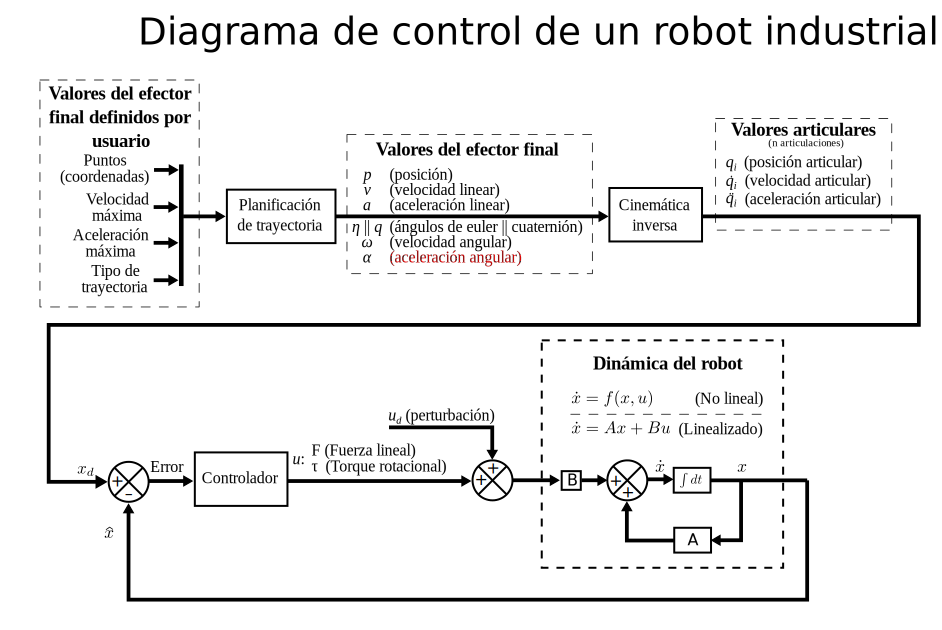
\includegraphics[width=\linewidth]{img/Diagrama_robot_industrial}
	\caption{Diagrama de bloques de un robot industrial}
	\label{fig:diagrama-de-robot-industrial}
\end{figure}

		
		\input{capitulos/Desarrollo/Simulación}
	
	% Capítulo 4: Resultados
	\chapter{Resultados} \label{chap:resultados}
En la Figura~\ref{fig:CinematicaDirecta} se presentan los resultados obtenidos mediante la simulación en MATLAB de la cinemática directa del robot. La subfigura (a) muestra la configuración espacial del robot en un instante determinado, con la representación de sus articulaciones y eslabones en un entorno tridimensional. Esto permitió verificar visualmente que las posiciones alcanzadas por el efector final corresponden con los valores calculados a partir de los ángulos articulares.

La subfigura (b) muestra un conjunto de gráficas correspondientes a la evolución temporal de diversas variables cinemáticas. Se observa la trayectoria del efector final en los ejes $X$, $Y$ y $Z$, así como sus velocidades y aceleraciones lineales. También se incluyen las gráficas de orientación (ángulos de Euler), velocidades angulares y aceleraciones angulares, las cuales son consistentes con un movimiento continuo y sin cambios bruscos.

Además, se realizó la simulación en los entornos \textit{Gazebo} y \textit{RViz}, donde se implementó el modelo del robot y se le aplicó la trayectoria previamente calculada. En ambos entornos se observó un comportamiento correcto: el robot sigue la trayectoria deseada sin colisiones ni movimientos erráticos. Esto valida la precisión del modelo cinemático directo y la correcta implementación de los ángulos de las juntas. La correspondencia entre los resultados visuales y los obtenidos en las gráficas refuerza la confiabilidad de la simulación realizada.

\begin{figure}[H]
	\centering
	\begin{minipage}[t]{0.49\textwidth}
		\centering
		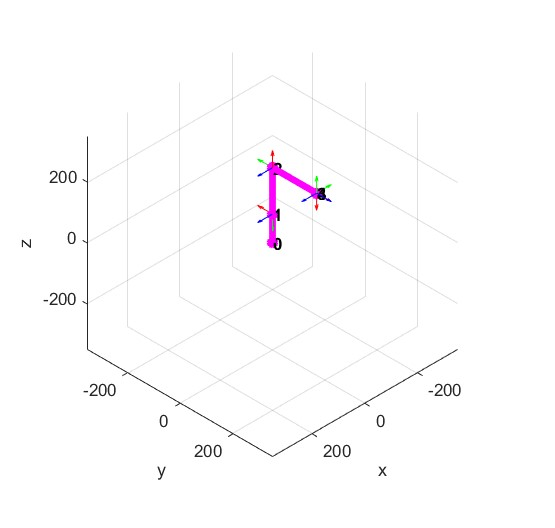
\includegraphics[width=\linewidth]{NuestroRobot_Directa.jpg}
		\caption*{(a) Configuración de juntas del robot}
	\end{minipage}
	\hfill
	\begin{minipage}[t]{0.49\textwidth}
		\centering
		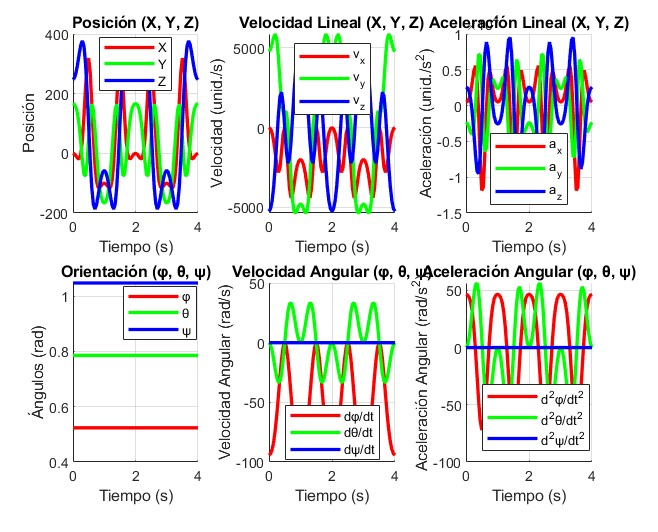
\includegraphics[width=\linewidth]{NuestroRobot_DirectaResultados.jpg}
		\caption*{(b) Resultados de la cinemática directa}
	\end{minipage}
	\caption{Cinemática directa del robot: configuración de juntas y resultados}
	\label{fig:CinematicaDirecta}
\end{figure}

En la Figura~\ref{fig:simulacion_gazebo} se observa al robot modelado en el entorno \textit{Gazebo}, donde se lleva a cabo una simulación física que incluye efectos como la gravedad, colisiones y dinámica. Esta simulación permitió verificar que el robot sigue correctamente la trayectoria establecida, sin desviaciones, oscilaciones anómalas ni interferencias con el entorno.

\begin{figure}[H]
	\centering
	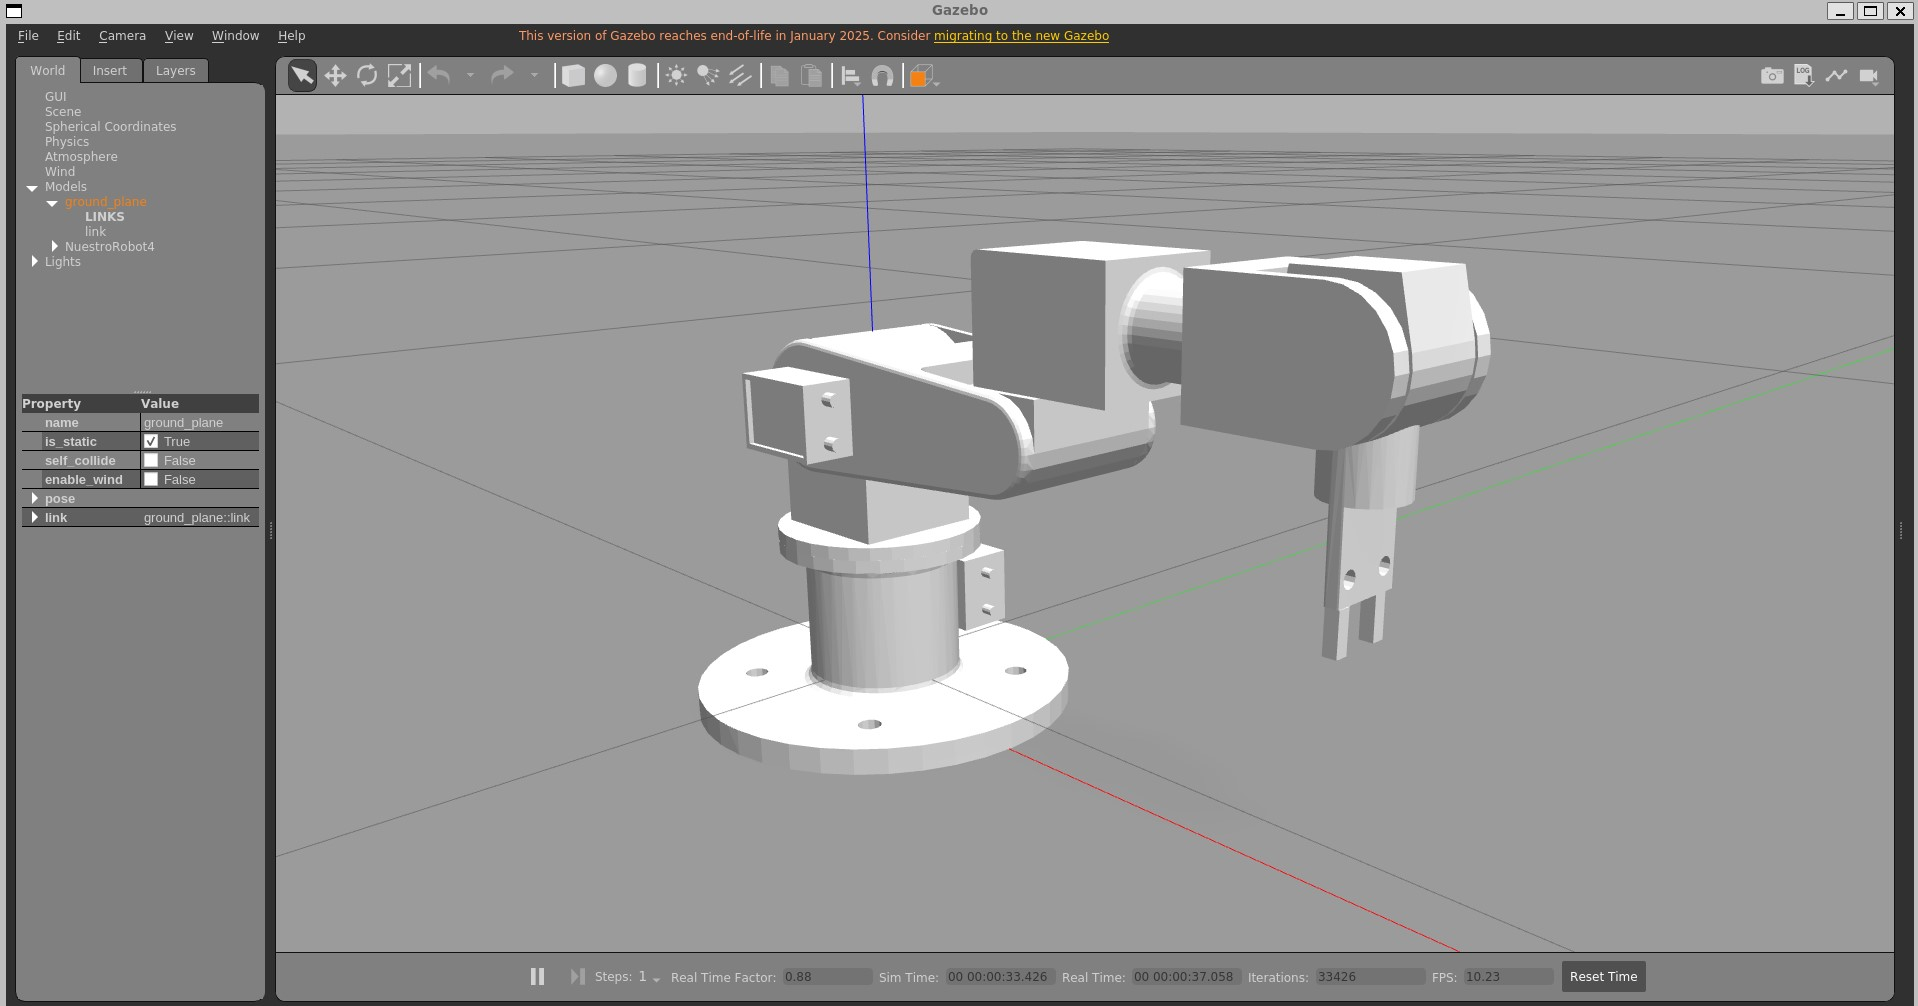
\includegraphics[width=0.8\textwidth]{Gazebo.jpg}
	\caption{Simulación del robot en el entorno Gazebo}
	\label{fig:simulacion_gazebo}
\end{figure}

En la Figura ~\ref{fig:GazeboYrviz} se presenta una vista combinada del robot en \textit{Gazebo} y \textit{RViz}. Mientras que Gazebo ejecuta la física de la simulación, RViz permite la visualización en tiempo real de los datos publicados por los nodos ROS, incluyendo la cinemática del robot y la trayectoria del efector final. En esta visualización, se confirma que el modelo de RViz reproduce de manera precisa los movimientos generados en Gazebo, lo cual indica que la cinemática directa y la publicación de transformaciones se implementaron correctamente.

Ambos entornos muestran que el robot cumple con el objetivo de seguir la trayectoria deseada, validando la correcta integración del modelo cinemático y su ejecución en ROS.


\begin{figure}[H]
	\centering
	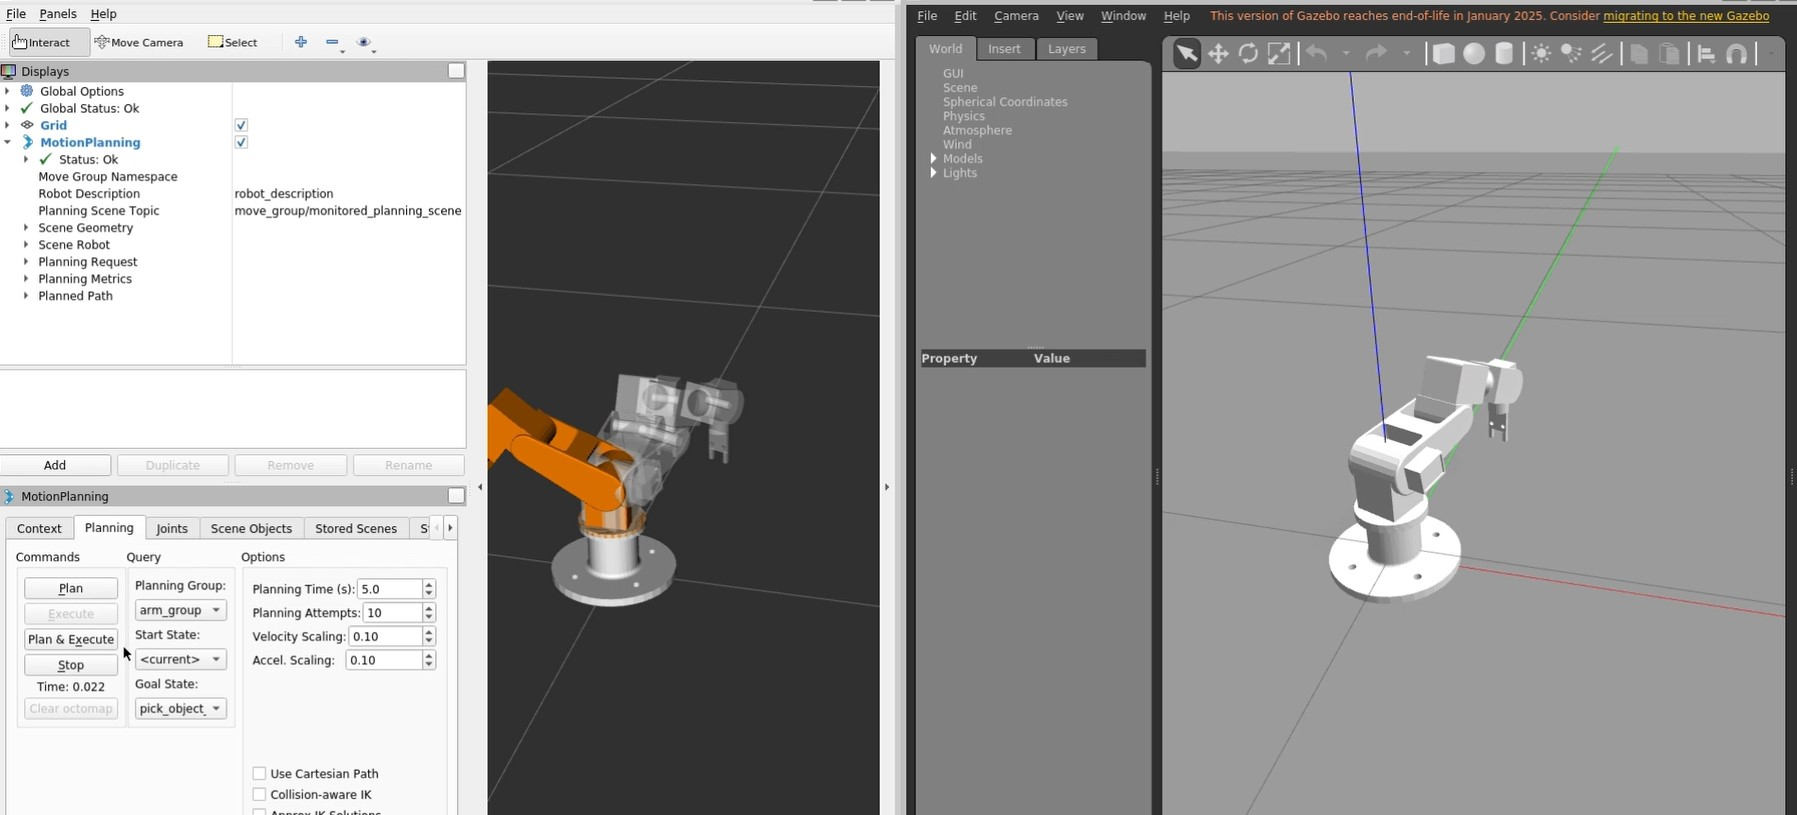
\includegraphics[width=0.8\textwidth]{GazeboRViz.jpg}
	\caption{Visualización del robot en RViz y Gazebo}
	\label{fig:GazeboYrviz}
\end{figure}

	
	% Capítulo 5: Conclusiones
	\chapter{Conclusiones} \label{sec:conclusiones}
	\section{Addiel Adrián Ocampo Ramos}
Este proyecto fue un reto de Verdad ya que estuvimos usando unos programas y lenguajes de programación el cual estábamos muy poco familiarizados con el. Tuvimos que investigar mucho para poder entender y comprender cómo podíamos crear nuestro robot, desde que empezamos usando el programa de solid works para crear lo que iba a ser el diseño de nuestro robot, ora luego pasar todo ese modelado en el programa ROS fue un reto la verdad ya que conocíamos muy poco ese software. Después de este tuvimos que investigar que material usaríamos en nuestro robot, usamos el método de Denavit-Hatenberg para determinar la cinemática de movimiento de nuestro robot y ser capaces de realizar los movimientos que se le necesiten hacer
	\section{Panchito}
Conclusiones y comentarios de Panchito, explicando los problemas que tuvo y lo que aprendió.
	\section{Sebastián Martínez Navarro}
Durante el desarrollo de este proyecto pudimos aplicar de manera práctica los conocimientos adquiridos en el curso de Robótica, particularmente en lo relacionado con la cinemática y dinámica de brazos robóticos.

Uno de los principales problemas fue el modelado cinemático e inverso, ya que se requería una buena interpretación del sistema de coordenadas y del método de Denavit-Hartenberg. También se me dificultó un poco el correr algunos programas en MATLAB ya que en momentos parecía hasta cosa de suerte para que corrieran bien los programas, sin embargo, eso mismo también considero que me ayudó a aprender a solucionar problemas y adentrarme más a la programación de MATLAB.

Otra limitación fue el espacio de mi laptop para descargar los programas así que agradezco que no todos los miembros del equipo tenían que tener todos los software y se logró repartir el trabajo en equipo de manera que todos aportaran en algun área, ya sea modelado, programación o redacción de reportes.

En cuanto a la teoría, fue un reto comprender e implementar las ecuaciones dinámicas del robot, ya que involucran conceptos avanzados como matrices de inercia, fuerzas de Coriolis y fricción, temas en los que no estaba muy familiarizado. 
Otro aspecto importante fue el trabajo en equipo. El uso de herramientas como GitHub y SourceTree, y LaTeX nos permitieron organizarnos mejor y entregar un trabajo más completo, para muchos (yo incluido) fue la primera vez que trabajamos con este tipo de programas, me parece muy bien aprenderlos ya que son herramientas muy comunes en la industria.


	\section{Pepito}
Conclusiones y comentarios de Pepito, explicando los problemas que tuvo y lo que aprendió.
		
	\titleformat{\chapter}
	{\bfseries\huge}
	{}
	{0pt}
	{~\raisebox{-1.5pt}{}
		\\\vspace{.05cm}\titlerule\\\filcenter #1 \\\vspace{.25cm}\titlerule}
	%{\titlerule\\\vspace{.25cm}\filcenter #1 \\\vspace{.25cm}\titlerule}
	\bibliographystyle{IEEEtranN}
	\newpage\label{bibliografia}
	\addcontentsline{toc}{chapter}{Bibliografía}
	
	% Pulsa Ctrl + Clic Izquierdo en bibliografia para entrar.
	\bibliography{bibliografia}
\end{document}


